\documentclass[11pt]{exam}

\usepackage{amssymb, amsmath, amsthm, mathrsfs, multicol, graphicx} 
\usepackage{tikz}

\def\d{\displaystyle}
\def\?{\reflectbox{?}}
\def\b#1{\mathbf{#1}}
\def\f#1{\mathfrak #1}
\def\c#1{\mathcal #1}
\def\s#1{\mathscr #1}
\def\r#1{\mathrm{#1}}
\def\N{\mathbb N}
\def\Z{\mathbb Z}
\def\Q{\mathbb Q}
\def\R{\mathbb R}
\def\C{\mathbb C}
\def\F{\mathbb F}
\def\A{\mathbb A}
\def\X{\mathbb X}
\def\E{\mathbb E}
\def\O{\mathbb O}
\def\pow{\mathscr P}
\def\inv{^{-1}}
\def\nrml{\triangleleft}
\def\st{:}
\def\~{\widetilde}
\def\rem{\mathcal R}
\def\iff{\leftrightarrow}
\def\Iff{\Leftrightarrow}
\def\and{\wedge}
\def\And{\bigwedge}
\def\AAnd{\d\bigwedge\mkern-18mu\bigwedge}
\def\Vee{\bigvee}
\def\VVee{\d\Vee\mkern-18mu\Vee}
\def\imp{\rightarrow}
\def\Imp{\Rightarrow}
\def\Fi{\Leftarrow}

\def\={\equiv}
\def\var{\mbox{var}}
\def\mod{\mbox{Mod}}
\def\Th{\mbox{Th}}
\def\sat{\mbox{Sat}}
\def\con{\mbox{Con}}
\def\bmodels{=\joinrel\mathrel|}
\def\iffmodels{\bmodels\models}
\def\dbland{\bigwedge \!\!\bigwedge}
\def\dom{\mbox{dom}}
\def\rng{\mbox{range}}
\DeclareMathOperator{\wgt}{wgt}

\def\circleA{(-.5,0) circle (1)}
\def\circleAlabel{(-1.5,.6) node[above]{$A$}}
\def\circleB{(.5,0) circle (1)}
\def\circleBlabel{(1.5,.6) node[above]{$B$}}
\def\circleC{(0,-1) circle (1)}
\def\circleClabel{(.5,-2) node[right]{$C$}}
\def\twosetbox{(-2,-1.5) rectangle (2,1.5)}
\def\threesetbox{(-2,-2.5) rectangle (2,1.5)}


\def\bar{\overline}

%\pointname{pts}
\pointsinmargin
\marginpointname{pts}
\marginbonuspointname{pts-bns}
\addpoints
\pagestyle{headandfoot}
%\printanswers

\firstpageheader{Math 228}{\bf Homework 8}{} %Due: Wed, April 3}
\firstpagefooter{}{}{\footnotesize \em More $\rightarrow$}
\runningfooter{}{}{}

\def\vertexsize{4pt}
\newcommand{\vtx}[2]{node[fill,circle,inner sep=0pt, minimum size=\vertexsize,label=#1:#2]{}}
\newcommand{\va}[1]{\vtx{above}{#1}}
\newcommand{\vb}[1]{\vtx{below}{#1}}
\newcommand{\vr}[1]{\vtx{right}{#1}}
\newcommand{\vl}[1]{\vtx{left}{#1}}
\renewcommand{\v}{\vtx{above}{}}

\begin{document}
\noindent \textbf{Instructions}: Same rules as usual - turn in your work on separate sheets of paper.  You must justify all your answers for full credit.

\begin{questions}

\question[8] For each sequence given below, find a closed formula for $a_n$, the $n$th term of the sequence (assume the first terms are $a_0$) by relating it to another sequence for which you already know the formula.  In each case, briefly say how you got your answers.  
\begin{parts}
	\part 4, 5, 7, 11, 19, 35, \ldots
	\begin{solution}
		If we subtract 3 from each term, we get $1, 2, 4, 8, 16, 32, \ldots$, which are the powers of 2.  So we must shift this sequence up by 3 to get our sequence.  Thus
		\[a_n = 2^n + 3\]
	\end{solution}
	
	\part 0, 3, 8, 15, 24, 35, \ldots
	\begin{solution}
		Add 1 to each term - we get $1, 4, 9, 16, 25, 36, \ldots$, the square numbers.  So maybe our sequence as formula $a_n = n^2 - 1$.  Does this work?  $a_3 = 8$.  That is a term of our sequence, but it should be $a_2$.  So we want 
		\[a_n = (n+1)^2 - 1\]
	\end{solution}
	
	\part 6, 12, 20, 30, 42, \ldots
	\begin{solution}
		Each term is even, so let's see what happens when we divide by 2: we get $3, 6, 10, 15, 21,\ldots$.  These are the triangle numbers, but starting at $T_2$.  We know $T_n = \frac{n(n+1)}{2}$. We want $a_0 = 2T_2$, $a_1 = 2T_3$, and so on.  In general, $a_n = 2T_{n+2}$, so 
		\[a_n = (n+2)(n+3)\]
		(This is like a shift by 2 units to the left and a stretch by a factor of 2.)
	\end{solution}
	
	\part 0, 2, 7, 15, 26, 40, 57, \ldots (Cryptic Hint: these might be called ``house numbers'')
	\begin{solution}
		How far off from triangular number are these?  The triangular numbers (starting with $T_0$) are $0, 1, 3, 6, 10, 15, 21, \ldots$.  The given sequence differs from this by $0, 1, 4, 9, 16, 25, 36, \ldots$ the square numbers!  Thus
		\[a_n = \frac{n(n+1)}{2} + n^2\]
	\end{solution} 
\end{parts} 

\question[8] Starting with any rectangle, we can create a new, larger rectangle by attaching a square to the longer side.  For example, if we start with a $2\times 5$ rectangle, we would glue on a $5\times 5 $ square, forming a $5 \times 7$ rectangle:

\begin{center}
	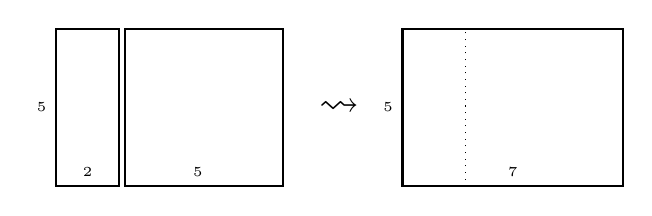
\begin{tikzpicture}[scale=.4]
		\draw[thick] (0,0) rectangle (2,5);
		\draw[thick] (2.2,0) rectangle (7.2,5);
		\draw (0,2.5) node[left]{\tiny 5} (1,0) node[above]{\tiny 2} (4.5,0) node[above]{\tiny 5};
		\draw (9,2.5) node{\Large $\rightsquigarrow$};
		\draw[thick] (11,0) rectangle (18,5);
		\draw[dotted] (13,0) -- (13,5);
		\draw (11,2.5) node[left]{\tiny 5}  (14.5,0) node[above]{\tiny 7};
	\end{tikzpicture}
\end{center}

\begin{parts}
	\part Create a sequence of rectangles using this rule starting with a $1\times 2$ rectangle.  Then write out the sequence of {\em perimeters} for the rectangles (the first term of the sequence would be 6, since the perimeter of a $1\times 2$ rectangle is 6 - the next term would be 10).
	\begin{solution}
		The rectangles are $1 \times 2$, $2 \times 3$, $3 \times 5$, $5 \times 8$, $8 \times 13$, and so on.  The sequence of perimeters is \[6, 10, 16, 26, 42, \ldots\]
	\end{solution}
	
	\part Repeat the above part this time starting with a $1 \times 3$ rectangle.
	\begin{solution}
		The sequence of rectangles have dimensions $1\times 3$, $3 \times 4$, $4 \times 7$, $7 \times 11$, $11\times 18$, and so on.  The sequence of perimeters is \[8, 14, 22, 36, 58, \ldots\]
	\end{solution}
	
	\part Find recursive formulas for each of the sequences of perimeters you found in parts (a) and (b).  Don't forget to give the initial conditions as well.
	\begin{solution}
		For the sequence from (a), the recursive formula is $a_1 = 6$, $a_2 = 10$, and $a_n = a_{n-1} + a_{n-2}$.
		
		For the sequence from (b), the recursive formula is $a_1 = 8$, $a_2 = 14$, and $a_n = a_{n-1} + a_{n-2}$.  
		
		Notice that both sequence have the same rule for getting terms from the previous ones, it is just the initial conditions that are different.  
	\end{solution}
	
	\part Are the sequences arithmetic?  Geometric?  If not, are they {\em close} to being either of these (for example, are the differences {\em almost} constant)?  Explain.
	\begin{solution}
		The sequences are not arithmetic because the differences between terms is not constant.  Similarly the ratio between terms is not constant, so the sequences are not geometric either.  
		
		However, look at the ratio between terms: $10/6 \approx 1.66$, $16/10 = 1.6$, $26/16 \approx 1.625$, $42/26 \approx 1.61$, \ldots.  In fact, the ratio between terms of the second sequence also floats around this same number.
		
		That number (and in fact, the limit of the ratios of either sequence as the terms increase) is $\frac{1 + \sqrt{5}}{2} \approx 1.618$, also known as the golden ratio.
		\end{solution}
\end{parts}

\question In their down time, ghost pirates enjoy stacking cannonballs in triangular based pyramids (aka, tetrahedrons), like those pictured here:

\centerline{\includegraphics[height=1in]{images/cannonballs.png}}

Note, in the picture on the right, there are some cannonballs (actually just one) you cannot see. The next picture would have 4 cannonballs you cannot see. 

The pirates wonder how many cannonballs would be required to build a pyramid 15 layers high (thus breaking the world cannonball stacking record).  Can you help?

\begin{parts}
\part[2] Let $P(n)$ denote the number of cannonballs needed to create a pyramid $n$ layers high.  So $P(1) = 1$, $P(2) = 4$, and so on.  Calculate $P(3)$, $P(4)$ and $P(5)$.
\begin{solution}
  To get the next larger pyramid, we add a triangle of cannonballs to the previous pyramid.  Thus to get $P(n)$, we add $P(n-1)$ to the $n$th triangular number:
  $P(3) = 4 + 6 = 10$, $P(4) = 10 + 10 = 20$, $P(5) = 20 + 15 = 35$.
\end{solution}


\part[4] Use polynomial fitting to find a closed formula for $P(n)$.  Show your work.
\begin{solution}
  The first differences are $3, 6, 10, 15, \ldots$.  The second differences are $3, 4, 5, 6, \ldots$.  The third differences are $1,1,1,\ldots$.  Since third differences are constant, we know the closed formula for $P(n)$ will be a degree 3 polynomial.  So $P(n) = an^3 + b n^2 + cn + d$.  Note that $P(0) = 0$, so $d = 0$.  To solve for $a$, $b$, and $c$, we solve the system of equations:
  \begin{align*}
    1 & = a + b + c \\
    4 & = 8a+ 4b + 2c \\
    10 & = 27a + 9b + 3c
  \end{align*}
  Doing so gives $a = \frac{1}{6}$, $b = \frac{1}{2}$ and $c = \frac{1}{3}$ so 
  \[P(n) = \frac{1}{6}n^3 + \frac{1}{2} n^2 + \frac{1}{3} n\]
\end{solution}


\part[2] Answer the pirate's question: how many cannonballs do they need to make a pyramid 15 layers high?

\begin{solution}
  \[P(15) = \frac{1}{6}15^3 + \frac{1}{2} 15^2 + \frac{1}{3} 15 = 680\]
\end{solution}

\end{parts}

\question[6] If you have enough toothpicks, you can make a large triangular grid.  Below, are the triangular grids of size 1 and of size 2.  The size 1 grid requires 3 toothpicks, the size 2 grid requires 9 toothpicks.

\centerline{\includegraphics[height=1in]{images/triangles.png}}
 
\begin{parts}
  \part Let $t_n$ be the number of toothpicks required to make a size $n$ triangular grid.  Write out the first 5 terms of the sequence $t_1, t_2, \ldots$.
  \begin{solution}
    $ 3, 9, 18, 30, 45, \ldots$
  \end{solution}

  \part Find a recursive definition for the sequence.  Explain why you are correct.
  \begin{solution}
    $t_n = t_{n-1} + 3n$.  This works because to get the next larger triangular grid, we must add a row of $n$ triangles, each requiring 3 toothpicks.
  \end{solution}

  \part Find a closed formula for the sequence.  Explain why you are correct.
  \begin{solution}
    You could do this using polynomial fitting, but there is an easier way - notice that each term in the sequence is a multiple of 3.  Dividing each term by 3 gives the sequence $1,3, 6, 10, 15,\ldots$ - the triangular numbers. This makes sense because we are forming triangles out of 3-toothpick collections.   So a closed formula is therefore
    $t_n = 3\frac{n(n+1)}{2}$
  \end{solution}

\end{parts}

\bonusquestion[4] Bonus: How many triangles (of all sizes and orientations) are contained in a size $n$ triangular grid?  For example, there is one triangle in a size 1 grid, and 5 triangles in a size 2 grid.
\begin{solution}
  To count the triangles, you need to separate the upright triangles from the upside down triangles.  The upright triangles are counted as the sum of triangular numbers, so should be described by a degree 3 polynomial.  The formula for upside down triangles is harder - the formula will be slightly different depending on whether $n$ is even or odd.
\end{solution}



\end{questions}




\end{document}

%\question[4] We have a formula $n$th term of an arithmetic sequence with first term $a$ and common difference $d$.  It is $a_n = a+d(n-1)$.  Find a closed formula for the \underline{sum} of the first $n$ terms of the sequence: $S_n = a_1 + a_2 + \cdots + a_n$.  Show your work.
%
%\begin{solution}
%  \begin{align*}
%    S = &~ a + (a+d) + (a+2d) + \cdots + (a+d(n-1))\\
%    \underline{+ S    = }& \underline{~(a+d(n-1)) + (a+d(n-2)) + \cdots + (a+d) + a}\\
%    2S  = &(2a + d(n-1)) + (2a + d(n-1)) + \cdots + (2a + d(n-1))\\
%    2S  = &(2a + d(n-1))n \mbox{~~~~ {\footnotesize b/c there are $n$ terms in the sum}}
%  \end{align*}
%Thus $S = \dfrac{(2a + d(n-1))n}{2}$
%\end{solution}
%
%
%\question[4] The $n$th term of a geometric sequence with first term $a$ and common ratio $r$ is $a_n = a\cdot r^{n-1}$.  Find a close formula for the \underline{sum} of the first $n$ terms of the sequence: $S_n = a_1 + a_2 + \cdots + a_n$.  Show your work.
%
%\begin{solution}
%  \begin{align*}
%    S = &~ a + ar + ar^2 + ar^3 + \cdots + ar^{n-1} \\
%    \underline{- rS = }& \underline{~~~~~~ ar + ar^2 + ar^3 + \cdots + ar^{n-1} + ar^n}\\
%    S - rS = & ~ a - ar^n\\
%    S(1-r) = & ~ a(1 - r^n)
%  \end{align*}
%So $S = \dfrac{a(1-r^n)}{1-r}$
%\end{solution}
